\chapter{Optimierungen}
\label{chap:optimizer}
In diesem Kapitel wird beschrieben, welche Optimierungen für den Compiler implementiert wurden. Im Forth-Cross-Compiler sind schon einige Peephole-Optimierungen implementiert. In diesem Kapitel werden die neu implementierten Optimierungen mit denen des Cross-Compilers verglichen und es wird gezeigt, wo noch bessere Optimierungsstrategien verwendet werden können.

\section{Peephole-Optimierung}

Peephole-Optimierungen sind Optimierungen, die auf einer kleinen Sequenz von Instruktionen durchgeführt werden. Diese Sequenz wird Peephole oder auch Window genannt. Die Peephole-Optimierung versucht, Paare von Instruktionen durch kürzere oder schnellere Instruktionen zu ersetzen.\cite{peepwiki} Peephole-Optimierungen können den Code um 15--40 Prozent verkleinern und sind heute in allen gängigen Compilern implementiert.\cite{peepdavidson} Zu den Peephole Optimierungen gehören unter anderen folgende Arten von Optimierungen:

\begin{itemize} 
	\item Constant Folding - konstante Ausdrücke auswerten
	\item Constant Propagation - konstante Werte in Ausdrücken substituieren
	\item Strength Reduction - langsame Instruktionen durch äquivalente schnelle Instruktionen ersetzen
	\item Combine Operations - mehrere Operationen durch eine äquivalenten Operation ersetzen
	\item Null Sequences - unnötige Operationen entfernen\cite{peepwiki}
\end{itemize}

\newpage

\subsection{Beispiele}

Einige Beispiele von Peephole-Optimierungen in Forth Code.

\subsubsection{Constant Propagation}
\label{constantprogationsection}

Die Instruktionen
%
\begin{verbatim}
1
2
swap
+
dup
\end{verbatim}
%
können durch
%
\begin{verbatim}
3
3
\end{verbatim}
%
ersetzt werden. Die Instruktionen \verb!swap!, \verb!+! und \verb!dup! können schon beim Kompilieren durchgeführt werden.
\subsubsection{Combine Operations}
Die Instruktionen
%
\begin{verbatim}
rot
rot
\end{verbatim}
%
können durch
%
\begin{verbatim}
-rot
\end{verbatim}
%
ersetzt werden. Die zwei \verb!rot! Instruktionen sind äquivalent zu einer \verb!-rot!-Instruktion. \\Die Instruktionen
%
\begin{verbatim}
dup
drop
\end{verbatim}
%
können durch
%
\begin{verbatim}
nop
\end{verbatim}
%
ersetzt werden. Die zwei Instruktionen \verb!dup! und \verb!drop! heben sich auf und können somit entfernt werden.

\newpage

\subsection{Optimierungen}

Für den Compiler wurden zwei Peephole-Optimierungs Prototypen in Java implementiert. Die erste Optimierung versucht benachbarte Instruktionen zu vereinfachen. Die zweite Optimierung ist eine einfache Constant Propagation. Die beiden Optimierungen werden in den nächsten Kapiteln genauer beschrieben. Der neue Optimizer wird in zwei Phasen durchgeführt:

\begin{figure}[H]
	\centering
		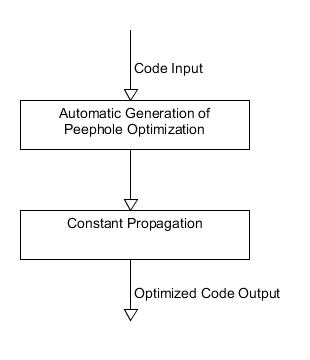
\includegraphics[scale=0.6]{optimizer/optimizer.png}
		\caption{Die zwei Phasen des Optimizers.}
		\captionsetup{margin=0cm,font={footnotesize}}
		\label{fig:optimizer}
\end{figure}

Im Cross-Compiler wurden unter anderem folgende Peephole-Optimierungen schon implementiert.

\begin{enumerate}
  \item \verb!<lit> + ld, <lit> + st, <lit> + @!, and \verb!<lit> + !! werden durch automatisch inkrementierende Speicherzugriffsinstruktionen ersetzt, wenn \verb!<lit>! sich zwischen --4 und 3 befindet
  \item Die Patterns \\
					$ swap, over \rightarrow tuck$\\
					$	over, swap \rightarrow under$\\
					$	swap, drop \rightarrow nip$\\
					$	r>, >r \rightarrow nop$\\
				werden vom Forth-Cross-Compiler erkannt und optimiert\\
\end{enumerate}


Für eine komplette Liste siehe "`uForth real time, object oriented with debugger"' \cite{uforth}.

\newpage
\subsection{Automatische Generierung von Peephole Optimierungen}

Klassische Peephole Optimizer versuchen häufig, einige maschinenspezifische Patterns zu korrigieren. Der von Davidson und Fraser\cite{peepdavidson} beschriebene Algorithmus (PO) verwendet eine Machine Description, simuliert benachbarte Instruktionen und versucht, diese durch äquivalente, schnellere Instruktionen zu ersetzen. Für den Forth-Optimizer wurde ein Teil von PO objektorientiert implementiert.

\subsection{Constant Propagation}
Unter Constant Propagation versteht man das Vorwärtssubstituieren von Konstanten im Code. Dies kann zur Folge haben, dass mehrere Instruktionen schon beim Kompilieren ausgewertet werden können, wie die Beispiele \ref{constantprogationsection} zeigen.

\subsection{Resultate und Tests}
Die Resultate des Optimierers wurden mit verschiedenen Forth-Funktionen getestet und mit dem Peephole-Optimizer des uForth-Cross-Compilers verglichen. Der Source Code zu den getesteten Funktionen befindet sich im Anhang.

\begin{table}[H]
\begin{center}
    \begin{tabular}{ | l | l | l | l | p{8cm} |}
    \hline
    \textbf{Funktion} & \textbf{Orig} & \textbf{Ref} & \textbf{Neu} & \textbf{Kommentar} \\ \hline
    \_Init & 126 & 112 & 119 & Die Referenzimplementierung produziert vor allem wegen der Speicherzugriffsoptimierung kürzeren Code. Constant Propagation, die neu implementiert wurde, konnte keine durchgeführt werden. PO konnte Instruktionspaare finden, die vereinfacht werden können.  \\ \hline
		\_Update & 8 & 8 & 4 & PO konnte zwei Instruktionspaare vereinfachen, welche von der Referenzimplementierung nicht optimiert werden. \\ \hline
		\_Hash & 65 & 60 & 60 & Die Referenzimplementierung produziert wegen der Speicherzugriffsoptimierung weniger Code. PO konnte Instruktionspaare finden, welche vereinfacht werden können. \\ \hline
		\_Propagation & 11 & 11 & 4 & Bei dieser Funktion konnte vor allem Constant Propagation durchgeführt werden. Die Referenzimplementierung führt keine Constant Propagation durch und konnte somit nichts vereinfachen. \\ \hline
    \end{tabular}
		\caption{Resultate des neuen Optimizers verglichen mit dem Cross-Compiler Optimizer.}
		\label{tab:peepresults}
\end{center}
\end{table}
\newpage

Es hat sich herausgestellt, dass bei allen Beispielen die Constant Propagation nur wenig Code optimieren konnte. Dies ist vermutlich der Fall, weil konstante Ausdrücke schon vom Compiler optimiert werden und die implementierte Constant Propagation zu primitiv ist. Im nächsten Kapitel werden einige Erweiterungen vorgeschlagen, um die Constant Propagation effizienter zu gestalten.  

PO konnte Regeln finden, die vom Forth-Cross-Compiler nicht erkannt werden. Unter anderem folgende:\\ \\
%
$swap, swap \rightarrow nop$\\
$-rot, rot \rightarrow nop$\\
$rot, -rot \rightarrow nop$\\
$1, + \rightarrow 1+$\\
$swap, + \rightarrow +$\\
%

Diese Regeln könnten in dem Forth-Cross-Compiler integriert werden. Im nächsten Kapitel werden Änderungen für den PO vorgeschlagen, damit dieser mehr Instruktionspaare, die vereinfacht werden können, erkennt.

\subsection{Mögliche Erweiterungen}

Im Moment werden vom PO nur Instruktionen simuliert, die einen Einfluss auf den Daten-Stack haben. PO könnte erweitert werden, indem auch andere Instruktionen simuliert werden, um mögliche Vereinfachungen zu finden. Eine weitere Möglichkeit wäre, den von Bansal und Aiken beschriebene Superoptimizer zu implementierten. Dieser Superoptimizer verwendet Bruteforce-Optimierungen mit tausenden von Regeln. Diese Regeln werden von Trainingsprogrammen inferiert und in einer Datenbank gespeichert.\cite{superoptimizer}

Die Constant Propagation könnte so erweitert werden, dass sie auch mit Branches umgehen kann. Somit könnten unnötige If-Statements und Schleifen entfernt werden. Um dies zu implementieren müsste der Code zuerst in eine Static Single Assignemt Form (SSA) transformiert werden.\cite{ssa} Es wäre dann jedoch keine Peephole-Optimierung mehr.